\chapter{Background and Preliminaries}\label{ch:background}

This chapter fixes the notation used in the rest of the report. It describes how the models in this report are sampled (\cref{sec:bg-flow}), the anatomy of a diffusion transformer (\cref{sec:bg-dit}), the residual-caching formulation shared by ReSPect and KalSea (\cref{sec:bg-residual}), the spectrally aligned gate (\cref{sec:bg-sea}), and the metrics and protocol used to evaluate a cache (\cref{sec:bg-metrics}).

%% ------------------------------------------------------------------------------------------------
\section{Sampling diffusion and flow-matching models}\label{sec:bg-flow}

\paragraph{Flow matching.} Rectified-flow models \citep{lipman2023flow,liu2023rectifiedflow,albergo2023stochastic,esser2024sd3} interpolate linearly between a data sample $x_\star$ and Gaussian noise $\epsilon\sim\mathcal N(0,I)$,
\begin{equation}
  x_\sigma = (1-\sigma)\,x_\star + \sigma\,\epsilon, \qquad \sigma\in[0,1],
\end{equation}
and train a network $v_\theta(x_\sigma,\sigma,c)$ to predict the velocity $\epsilon - x_\star$ for a condition $c$ (e.g.\ a text prompt). Sampling starts from pure noise and integrates the learned velocity over a decreasing schedule $\sigma_0>\sigma_1>\dots>\sigma_N=0$ with Euler steps,
\begin{equation}\label{eq:bg-euler}
  x_{i+1} = x_i + (\sigma_{i+1}-\sigma_i)\, v_i, \qquad v_i = v_\theta(x_i,\sigma_i,c), \qquad i=0,\dots,N-1 .
\end{equation}
FLUX.1-dev uses this sampler with $N=50$ and a resolution-dependent shift of the schedule. Each step costs one evaluation of the network, so a sample costs $N$ network function evaluations (NFE).

\paragraph{Variance-preserving diffusion and DDIM.} DDPM-type models \citep{ho2020ddpm} define $x_t = \sqrt{\bar\alpha_t}\,x_0 + \sqrt{1-\bar\alpha_t}\,\epsilon$ for a decreasing signal level $\bar\alpha_t$. With the network predicting $\hat\epsilon$, $\hat x_0$, or the ``velocity'' $v = \sqrt{\bar\alpha_t}\epsilon - \sqrt{1-\bar\alpha_t}x_0$ \citep{salimans2022progressive}, the deterministic DDIM update \citep{song2021ddim} from $t$ to the previous timestep $t'$ is
\begin{equation}\label{eq:bg-ddim}
  x_{t'} = \sqrt{\bar\alpha_{t'}}\,\hat x_0 + \sqrt{1-\bar\alpha_{t'}}\,\hat\epsilon ,
\end{equation}
which, for every one of these parametrisations, is an \emph{affine} function of the network output: $x_{t'} = A_t x_t + B_t\, v_\theta(x_t,t)$. This linearity is all that KalSea's corrector needs (\cref{ch:kalsea}). Multistep solvers such as UniPC \citep{zhao2023unipc} combine several past outputs, but remain linear in the outputs for a fixed solver state.

\paragraph{Signal and noise coefficients.} Both families can be written as $x_t = a_t x_0 + b_t\epsilon$, with $(a_t,b_t)=(1-\sigma,\sigma)$ for flow matching and $(\sqrt{\bar\alpha_t},\sqrt{1-\bar\alpha_t})$ for variance-preserving diffusion. These coefficients are read from the sampler and determine the spectral filter of the gate (\cref{sec:bg-sea}).

%% ------------------------------------------------------------------------------------------------
\section{Anatomy of a diffusion transformer}\label{sec:bg-dit}

A diffusion transformer \citep{peebles2023dit} computes the network output in three stages:
\begin{equation}\label{eq:bg-stages}
  h^{\mathrm{in}}_i = \Emb(x_i), \qquad h^{\mathrm{out}}_i = F\big(h^{\mathrm{in}}_i, c_i\big), \qquad v_i = \Out\big(h^{\mathrm{out}}_i, c_i\big),
\end{equation}
where $\Emb$ embeds the latent patches into tokens, $F$ is the stack of transformer blocks, $\Out$ is a final adaptive normalisation followed by a linear projection back to latent patches, and $c_i$ embeds the timestep (and, for FLUX.1-dev, the guidance scale and pooled text). Each block modulates its inputs with adaptive layer normalisation:
\begin{equation}\label{eq:bg-adaln}
  \mathrm{AdaLN}(h, c) = \big(1+\gamma(c)\big)\odot\mathrm{LayerNorm}(h) + \beta(c),
\end{equation}
with scale $\gamma$ and shift $\beta$ regressed from $c$. In FLUX.1-dev, $F$ consists of 19 double-stream blocks, which keep separate image and text streams that interact through joint attention, followed by 38 single-stream blocks over the concatenated sequence; a $1024\times1024$ image corresponds to $64\times 64 = 4096$ image tokens. Almost all of the computation is in $F$; $\Emb$ and $\Out$ together cost a fraction of a percent of one evaluation. This asymmetry is what makes residual caching, and KalSea's corrector, cheap.

%% ------------------------------------------------------------------------------------------------
\section{Residual caching}\label{sec:bg-residual}

A residual cache stores the block-stack residual of the image tokens on computed steps,
\begin{equation}\label{eq:bg-residual}
  r_i = h^{\mathrm{out}}_i - h^{\mathrm{in}}_i ,
\end{equation}
and on skipped steps runs only $\Emb$ and $\Out$:
\begin{equation}\label{eq:bg-skip}
  \hat h^{\mathrm{out}}_j = h^{\mathrm{in}}_j + \hat r_j, \qquad \hat v_j = \Out\big(\hat h^{\mathrm{out}}_j, c_j\big),
\end{equation}
where the \emph{filler} $\hat r_j$ is the last computed residual (reuse, as in TeaCache and SeaCache) or a forecast (ReSPect, KalSea). Because $h^{\mathrm{in}}_j$ is computed exactly from the current latent, the reconstruction error of the block-stack output equals the error of the filler:
\begin{equation}\label{eq:bg-error}
  \hat h^{\mathrm{out}}_j - h^{\mathrm{out}}_j = \hat r_j - r_j .
\end{equation}
\Cref{fig:bg-residual} illustrates one computed and one skipped step. Note that the sampler still advances the latent on skipped steps (\cref{eq:bg-euler}) with the approximate velocity $\hat v_j$; any error of the filler is therefore integrated into the latent. This point is central to KalSea.

\begin{figure}[t]
  \centering
  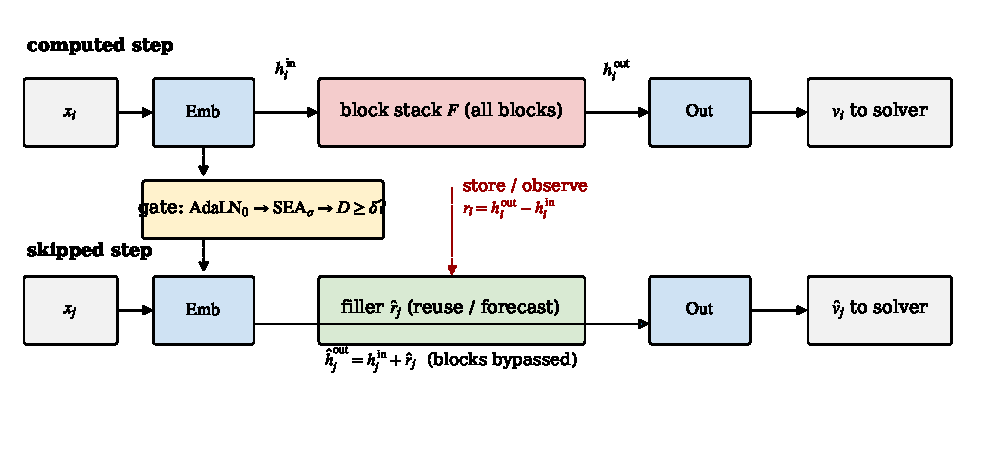
\includegraphics[width=0.92\textwidth]{bg_residual_cache.pdf}
  \caption[Residual caching]{Residual caching. On a computed step the full block stack $F$ runs and its residual $r_i = h^{\mathrm{out}}_i - h^{\mathrm{in}}_i$ is stored or observed. On a skipped step the blocks are bypassed: the filler $\hat r_j$ is added to the exactly computed input $h^{\mathrm{in}}_j$ and the result goes through the output layers. The gate decides which of the two paths a step takes.}
  \label{fig:bg-residual}
\end{figure}

%% ------------------------------------------------------------------------------------------------
\section{The spectrally aligned (SEA) gate}\label{sec:bg-sea}

\subsection{Gate input}
A gate must be evaluated at every step and must therefore be cheap. Following TeaCache \citep{liu2025teacache} and SeaCache \citep{chung2026seacache}, the gate reads the timestep-modulated input of the first block,
\begin{equation}
  I_i = \mathrm{AdaLN}_0\big(h^{\mathrm{in}}_i, c_i\big),
\end{equation}
which is available before any block runs and reflects both the latent and the noise level.

\subsection{Derivation of the Wiener response}
Model the latent at step $t$ as the linear mixture
\begin{equation}
  x_t = a_t x_0 + b_t \epsilon, \qquad \epsilon\sim\mathcal N(0,I),
\end{equation}
with $\epsilon$ white and independent of the clean latent $x_0$. This is a signal/noise model for the gate, not a claim about the exact forward process of each model. Consider the linear-MMSE estimator of $x_0$ from $x_t$, $h_t^\star = \arg\min_h \E\|h * x_t - x_0\|_2^2$. Assuming wide-sense stationarity, convolution is diagonal in the Fourier basis, and by Parseval's identity the risk of a filter with frequency response $H_t(f)$ splits per frequency:
\begin{equation}
  J_t(H_t) = \sum_f \Big[ |H_t(f)|^2\big(a_t^2S_x(f)+b_t^2\big) - 2\,\mathrm{Re}\big(H_t(f)\big)\,a_tS_x(f) + S_x(f)\Big],
\end{equation}
where $S_x$ is the power spectrum of $x_0$. Each summand is a scalar quadratic in $H_t(f)$; setting its derivative to zero gives $H_t(f)\big(a_t^2S_x(f)+b_t^2\big) = a_tS_x(f)$, i.e.\ the Wiener response \citep{wiener1949extrapolation}
\begin{equation}\label{eq:bg-wiener}
  G_t(f) = \frac{a_t\, S_x(f)}{a_t^2\, S_x(f) + b_t^2},
\end{equation}
which is a minimum because the second derivative $a_t^2S_x(f)+b_t^2$ is positive.

\paragraph{Spectral evolution.} Natural images follow a power law $S_x(f)\propto |f|^{-\beta}$ with $\beta\approx 2$. Inserting this prior into \cref{eq:bg-wiener}: at early steps ($a_t$ small) the denominator is dominated by the noise except near $f=0$, so $G_t$ is low-pass; as $a_t\to 1$ the passband widens towards high frequencies (\cref{fig:bg-wiener}a). This reproduces the coarse-to-fine evolution of diffusion sampling, in which global structure forms first and details later. SeaCache uses $\beta=2$ for images and $\beta=3$ for videos; for multi-dimensional token grids the filter is separable over the spatial (and temporal) axes.

\paragraph{Gain normalisation.} The raw responses differ by orders of magnitude in overall gain across steps, which would let high-gain steps dominate the accumulated distance. Each response is therefore normalised to unit mean gain over the frequency bins,
\begin{equation}\label{eq:bg-norm}
  G^{\mathrm{norm}}_t(f) = \nu_t\, G_t(f), \qquad \nu_t^{-1} = \frac{1}{L}\sum_{\ell} G_t(f_\ell),
\end{equation}
so that the accumulated distance measures changes of spectral shape rather than changes of filter gain (\cref{fig:bg-wiener}b).

\begin{figure}[t]
  \centering
  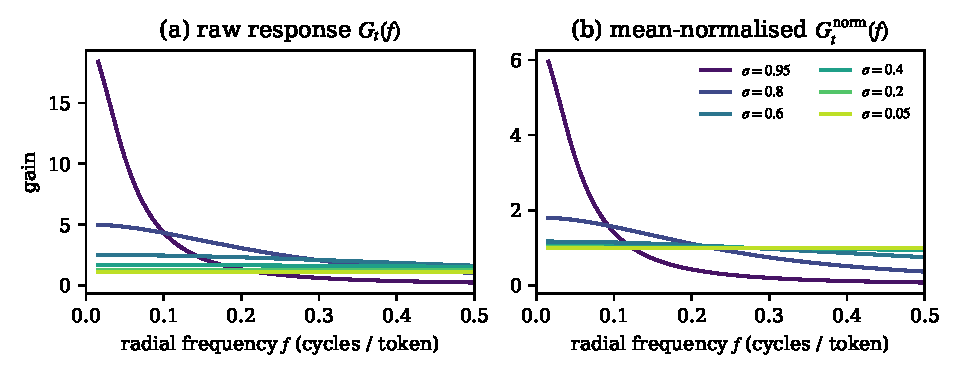
\includegraphics[width=0.95\textwidth]{bg_wiener.pdf}
  \caption[Wiener responses of the SEA filter]{Wiener responses of the SEA filter along a flow schedule ($a_t=1-\sigma$, $b_t=\sigma$, $S_x(f)=|f|^{-2}$), computed from the closed form of \cref{eq:bg-wiener}. (a) The raw response is low-pass at high noise and widens as $\sigma\to 0$. (b) After the mean-gain normalisation of \cref{eq:bg-norm}, the responses share a common scale and differ only in shape.}
  \label{fig:bg-wiener}
\end{figure}

\subsection{Accumulate-and-reset rule}
Let $\SEA_i(I) = \mathcal F^{-1}\big[G^{\mathrm{norm}}_{t_i}\odot\mathcal F(I)\big]$ denote the filtered gate input of step $i$ on its token grid. The gate computes the relative $\ell_1$ change between consecutive filtered inputs and accumulates it:
\begin{equation}\label{eq:bg-gate}
  d_i = \frac{\big\|\SEA_i(I_i) - \SEA_{i-1}(I_{i-1})\big\|_1}{\big\|\SEA_{i-1}(I_{i-1})\big\|_1}, \qquad D_i = D_{i-1} + d_i .
\end{equation}
Step $i$ is computed if $D_i\ge\delta$, after which $D_i$ is reset to zero, or if it is the first or the last step; otherwise it is skipped. The reference $\SEA_{i-1}(I_{i-1})$ is refreshed at \emph{every} step, computed or skipped, so that each $d_i$ measures only the incremental drift between consecutive solver states. The single threshold $\delta$ sets the compute budget: a larger $\delta$ skips more steps. Because the gate reads only the first block's modulated input, replacing the filler (reuse, ReSPect, KalSea) does not change where the gate fires, which allows fillers to be compared at an identical schedule.

%% ------------------------------------------------------------------------------------------------
\section{Evaluation methodology}\label{sec:bg-metrics}

\paragraph{Compute.} The compute of a cache is reported as the mean number of full block-stack evaluations per sample (NFE, out of 50 for the 50-step samplers), counted by hooks on the blocks. TFLOPs follow SeaCache's convention, and latency is the wall-clock time per sample on a single NVIDIA B200 GPU in bf16. Because a content-aware gate need not realise the same skip rate as another method at a shared $\delta$, methods are compared at \emph{matched or lower} compute, never at matched $\delta$.

\paragraph{Fidelity.} The goal of a cache is to reproduce the output of the uncached sampler. Every accelerated sample is therefore compared with the output of the uncached 50-step sampler for the same prompt and seed, using
\begin{itemize}
  \item \textbf{PSNR} on 8-bit RGB, $10\log_{10}(255^2/\mathrm{MSE})$ (higher is better);
  \item \textbf{SSIM} \citep{wang2004ssim}, the structural similarity index (higher is better);
  \item \textbf{LPIPS} \citep{zhang2018lpips}, a learned perceptual distance on AlexNet features (lower is better).
\end{itemize}
For videos the metrics are averaged over frames. In the KalSea study, differences between methods run in the same setup are reported with paired bootstrap 95\% confidence intervals over prompts (10{,}000 resamples, percentile method) and the fraction of prompts on which a method is better.

\paragraph{Benchmarks and models.} Text-to-image experiments use FLUX.1-dev \citep{bfl2024flux} at $1024\times1024$ with 50 steps, embedded guidance 3.5 and the 200 DrawBench prompts \citep{saharia2022imagen}, with the prompt index as seed. Text-to-video experiments use HunyuanVideo \citep{kong2024hunyuanvideo} and Wan2.1-T2V-1.3B \citep{wan2025wan} with 65 frames and 50 steps on VBench prompts \citep{huang2024vbench}. The exact settings of each study are given in \cref{ch:respect,ch:kalsea}.
